\section{Camera Extrinsic Calibration}
\label{section:camera-extrinsic-calibration}

The extrinsic parameters of the camera the position and orientation of the camera in the robot. In this case, the camera was mounted statically on top of the PTU, just like the laser scanner. This calibration that determines this extrinsic parameters is known as the eye-in-hand calibration, described in \cite{horaud95}.

This calibration relies on a static calibration object, whose pose can be estimated in the camera frame. Hence, four coordinate frames and four transformation exist. The four frames are the \emph{camera} frame, the \emph{world} frame, the \emph{PTU} frame and the \emph{object}. The four transformations are the extrinsic transformation of the camera, or the \emph{PTU} to the \emph{camera} transformation $\TF{ptu}{camera}$, which is static and unknown, the \emph{camera} to \emph{object} transformation $\TF{camera}{object}$, which is obtained by the object pose estimation algorithm, the \emph{world} to \emph{PTU}, which is known and, finally, the \emph{world} to \emph{object} transformation, which is static and unknown. The overall transformation graph is shown is in \cref{fig:hand-in-eye-tf-graph}, with the unknown transformations in red and the known transformations in green.

\begin{figure}
    
    \centering
    \begin{tikzpicture}
        \node[draw, ellipse] (world) at (0,0) {world};
        \node[draw, ellipse] (hand) at (-4,3) {hand/ptu};
        \node[draw, ellipse] (object) at (4,3) {object};
        \node[draw, ellipse] (camera) at (0, 6) {camera};
        
        \path[-latex]
            (world) edge[bend right] node[midway, below right, red] {$\TF{world}{object}$} (object)
            (world) edge[bend left] node[midway, below left, blue] {$\TF{world}{ptu}$} (hand)
            (hand) edge[bend left] node[midway, above left, red] {$\TF{hand}{camera}$} (camera)
            (camera) edge[bend left] node[midway, above right, blue] {$\TF{camera}{object}$} (object);
    \end{tikzpicture}

    \caption{Hand-in-eye transformation graph}
    \label{fig:hand-in-eye-tf-graph}

\end{figure}

The inspection of the transformation graph determines an equality, because there are two possible ways to transverse the graph from one node to another, which yields the \cref{eqn:hand-in-eye-equality}. This equality is the base of this optimization: $\TF{ptu}{camera}$ can be obtained from multiple pairs of synchronized $\TF{world}{object}$ and $\TF{camera}{object}$ transformations.

\begin{equation}
    \label{eqn:hand-in-eye-equality}
    \TF{world}{object} = \TF{world}{ptu} \cdot \TF{ptu}{camera} \cdot \TF{camera}{object}
\end{equation}

In this work, the object used for detection was an ArUco marker, which is comprised of a pattern which can be detected and also allows for precise pose estimation, as seen in \cref{fig:aruco-detection}. One of the biggest advantages over other markers is that the implementation for detection and pose estimation is already implemented in the ROS package \emph{aruco\_detect}. The calibration is also implemented in the ROS package \emph{visp\_hand2eye\_calibration}, as a node that receives multiple transformations in the topics \emph{/world\_effector} and \emph{/camera\_object}, which correspond respectively to the $\TF{world}{ptu}$ and $\TF{camera}{object}$ transformations. To publish the transformations on this topics, a node was developed, the \emph{hand2eye\_simple\_client}, which publishes both the transformations synchronously at the keypress of the user. The control of the PTU was also manual. 

\begin{figure}
    
    \centering
    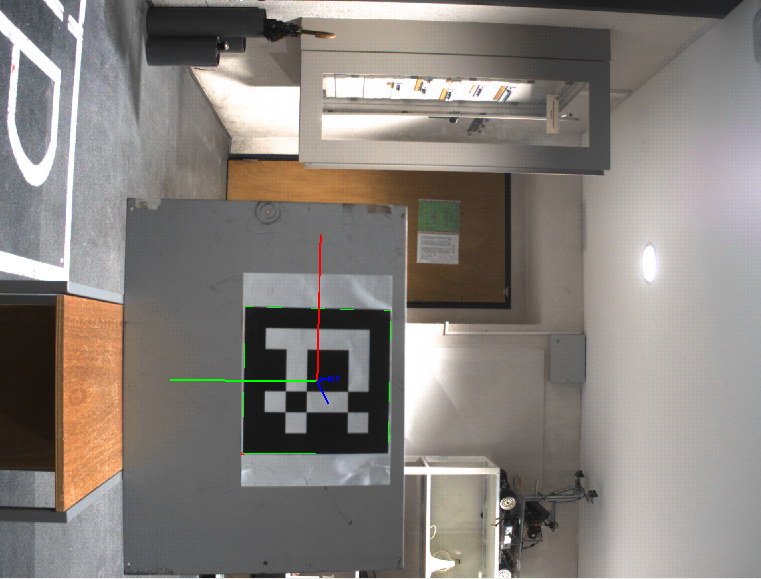
\includegraphics[width=10cm]{camera-extrinsic-calibration}

    \caption{ArUco maker detection and pose estimation.}
    \label{fig:aruco-detection}
\end{figure}